%\documentclass[10pt,handout]{beamer}
\documentclass[10pt]{beamer}
\usepackage{babel} % Anpassa efter svenska. Ger svensk logga.
\usepackage[utf8]{inputenc} % Anpassa efter linux
\usepackage{graphicx}
\usepackage{../common/beamerthemeUppsala}
%\usecolortheme{UU} % Anpassa efter UU:s frger och logga
%\hypersetup{pdfpagemode=FullScreen} % Adobe Reader ska ppna fullskrm
\setbeamertemplate{itemize items}[circle]

% \usepackage{beamerthemesplit}
\usepackage{amsmath}
\usepackage{amssymb}
% \usepackage{graphics}
% \usepackage{graphicx}
% \usepackage{epsfig}
% \usepackage[latin1]{inputenc}
 \usepackage{color}
% \usepackage{fancybox}
% \usepackage{psfrag}
% \usepackage[english]{babel}
 \setbeamertemplate{footline}{\hfill\insertframenumber/\inserttotalframenumber}


%library(tinytex)
%tlmgr_install('csquotes')
%\usepackage{csquotes}

% Read in commands
% Course settings
\newcommand{\currentsemester}{Autumn 2024}

% New commands
\newcommand{\bfm}[1]   {\mbox{\boldmath{${#1}$}}}
\newcommand{\Prob}   {\mbox{\textnormal{P}}}
\newcommand{\uured}[1]{\textcolor{uured}{#1}}

% Eqds
\def\eqd{\,{\buildrel d \over =}\,}

% Math operators
\DeclareMathOperator{\E}{\mathbb{E}}
\DeclareMathOperator{\V}{\mathbb{V}}


%%%%%%%%%%%%%%%%%%%%%%%%%%%%%%%%%%%%%%%%%%%%%%%%%%%%%%%%%%%%%%%%%%

\setlength{\parskip}{3mm}
\title[]{{\color{black}Machine learning -- Block 4}}
\author[]{M{\aa}ns Magnusson\\Department of Statistics, Uppsala University}
\date{\currentsemester}


\begin{document}

\frame{\titlepage
% \thispagestyle{empty}
}

%%%%%%%%%%%%%%%%%%%%%%%%%%%%%%%%%%%%%%%%%%%%%%%%%%%%%%%%%%%%%%%%%%


\begin{frame}{This week's lecture}
\begin{itemize}
\item Previous assignments
\item The Mini-Project and Master Thesis Projects
\item Convolutional Neural Networks
\item Transfer Learning
\end{itemize}
\end{frame}



%%%%%%%%%%%%%%%%%%%%%%%%%%%%%%%%%%%%%%%%%%%%%%%%%%%%%%%%%%%%%%%%%%

\section{Practicalities}

\begin{frame}{Assignment 3: Evaluation}

\begin{itemize}
\item A little bit to easy VG part.
\item How to think when building networks? Art and Science. Radom search and try to get as low training error as possible.
\item Keras lecture? Describe parameters?
\end{itemize}

\end{frame}

\begin{frame}{On this weeks assignment}
\begin{itemize}
\item It takes long time to run the models this week. Start early!
\end{itemize}
\end{frame}


\begin{frame}{Mini-project}

\begin{itemize}
\item Submission Tuesday (tomorrow) at 23.59!\pause
\item {\color{uured} Supervised} problem of choice on {\color{uured} real data}.\pause
\item 2-3 students.\pause
\item \emph{Hint!} Submit page 1 of the project as project proposal.
\item Feel free to combine it with your master thesis project!
\item Check with me if you have questions.
\item The project should result in a 4 page report (PDF) using the {\color{uured} ICML LaTeX template}.
\end{itemize}
\end{frame}

\begin{frame}{Master thesis projects}

\begin{itemize}
\item Still discussions... hopefully out today.
\end{itemize}
\end{frame}


\section{Introduction}
\frame{\sectionpage}

\frame{\frametitle{Convolutional Neural Networks}

\begin{itemize}
\item \uured{Acknowledgements}: Anders Eklund, Link\"{o}ping University.\pause
\item \uured{Convolutional} Neural Networks are behind great progress in the 2010s.
\item Revolutionized \uured{Computer Vision}.
\pause
\item Also called: ConvNets, Convolutional nets, Convolutional networks
\end{itemize}

\begin{figure}[h]
\caption{ImageNet performance (Roessler, 2019)}
\centering
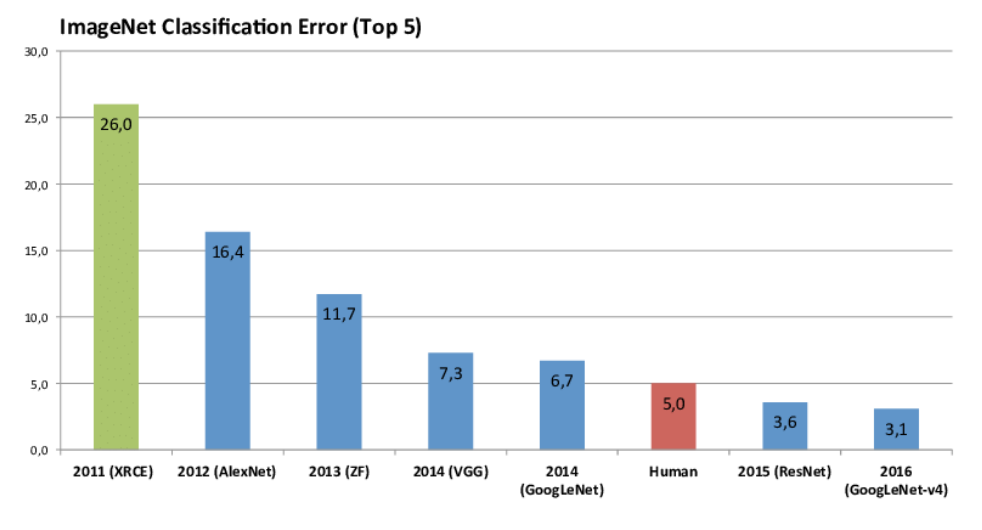
\includegraphics[width=0.8\textwidth]{fig/imageNet.png}
\end{figure}
\pause

}


\frame{\frametitle{Convolutional Neural Networks}

\begin{itemize}
\item Special architecture that works well for data with a \uured{grid structure}
\begin{enumerate}
\item 1D-grids: Time series\pause
\item 2D-grids: Gray-scale Images (pixels)\pause
\item 3D-grids: Color Images (pixels and chanels)\pause
\item 4D-grids: Color Video (pixels, chanels, frames)
\end{enumerate}
\end{itemize}

}

\frame{\frametitle{Computer Vision}

\begin{itemize}
\item Problems
\begin{itemize}
\item Image Classification\pause
\item Image Segmentation\pause
\item Object Detection\pause
\item Object Localization\pause
\end{itemize}
\item {\color{uured} Focus}: 2D and 3D data\pause
\item Very Large Datasets:
\begin{itemize}
\item ImageNet: 14M Images, 20k classes, 1M bounding boxes
\end{itemize}
\pause
\item Many different pre-trained models (e.g. VGG16)
\end{itemize}
}

\frame{\frametitle{Example: Object Detection}
\begin{figure}[h]
\centering
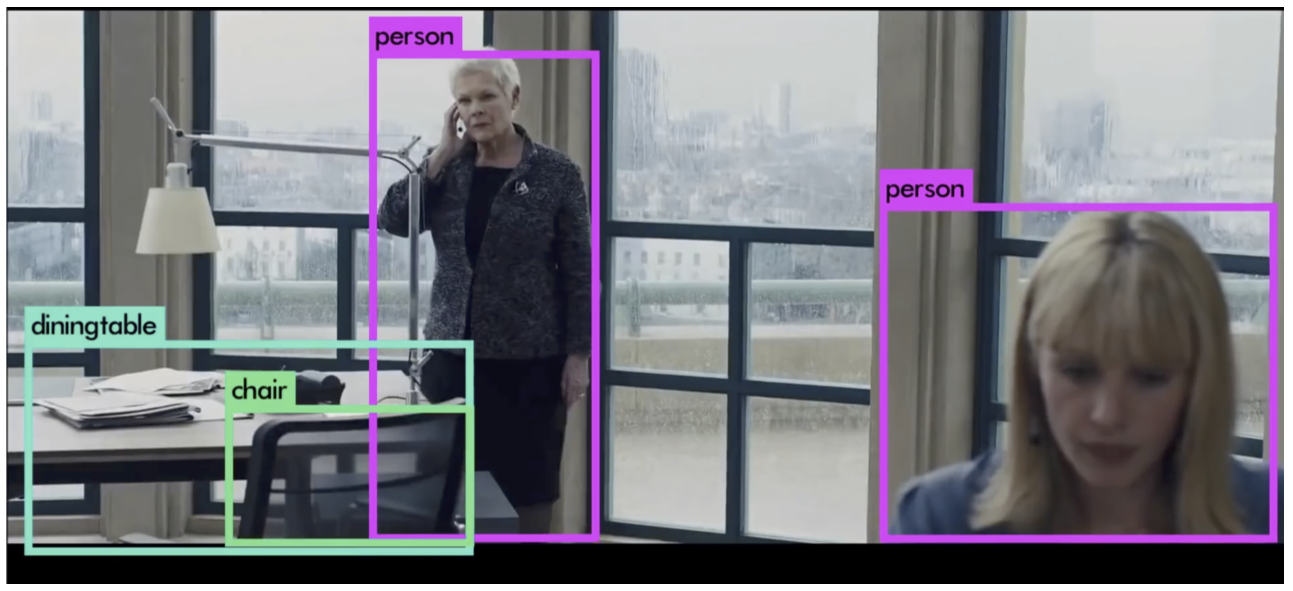
\includegraphics[width=0.8\textwidth]{fig/object_detection.png}
\caption{Object detection (see \href{https://www.youtube.com/watch?v=VOC3huqHrss}{https://www.youtube.com/watch?v=VOC3huqHrss}) }
\end{figure}
}

\frame{\frametitle{Example: Pneumonia detection}
\begin{figure}[h]
\centering
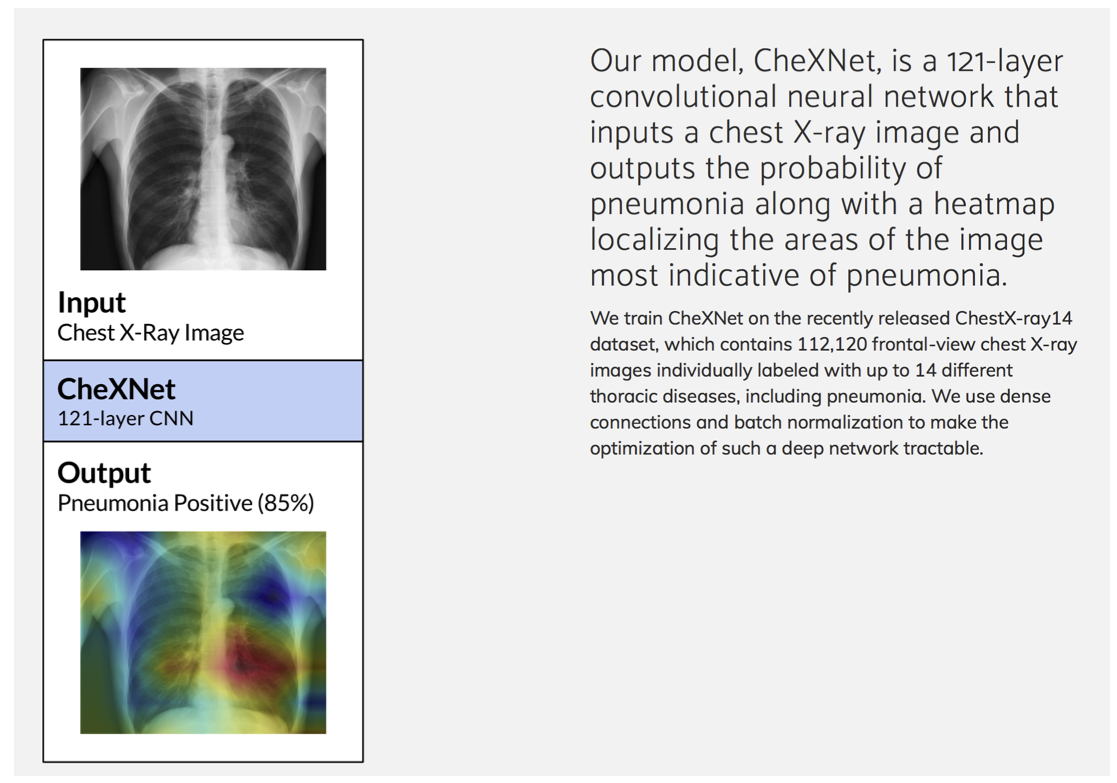
\includegraphics[width=0.8\textwidth]{fig/chexnet.png}
\caption{Rajpurkar et al. (2017). Chexnet: Radiologist-level pneumonia detection on chest x-rays with deep learning. arXiv preprint arXiv:1711.05225.}
\end{figure}
}

\frame{\frametitle{Example: Fracture detection}
\begin{figure}[h]
\centering
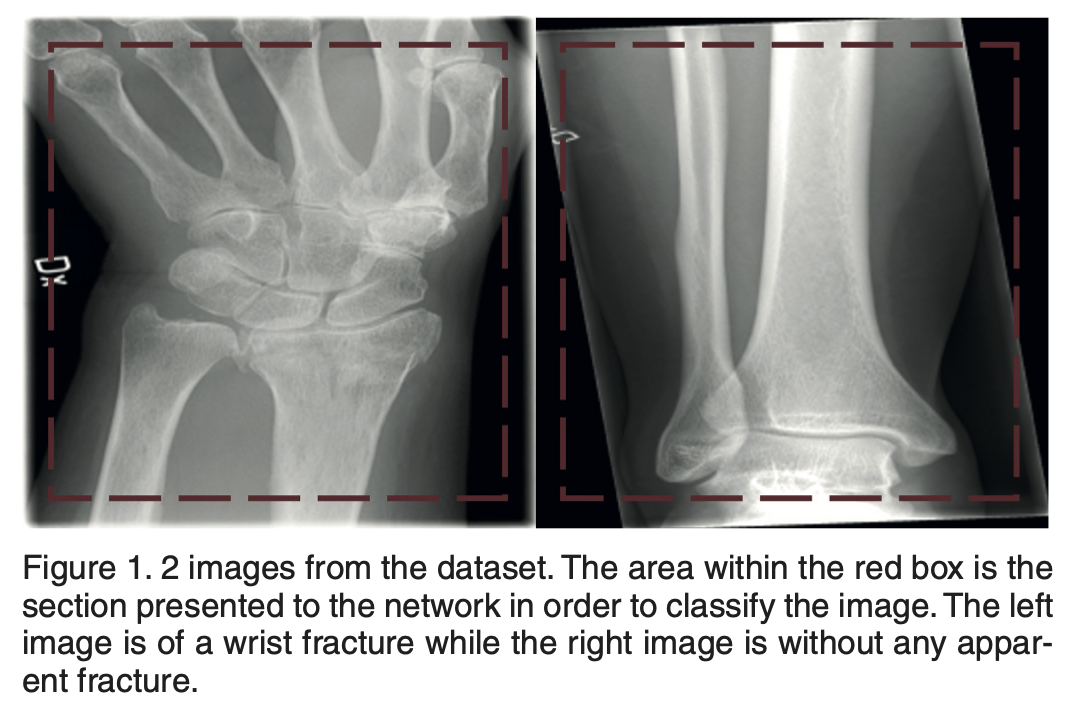
\includegraphics[width=0.8\textwidth]{fig/fractures.png}
\caption{Olczak et al, (2017) Artificial intelligence
for analyzing orthopedic trauma radiographs, Acta Orthopaedica, 88:6, 581-586}
\end{figure}
}


\frame{\frametitle{What is an Image?}

\begin{itemize}
\item 2-dimensional object
\item Each pixel has:
\begin{enumerate}
\item a coordinate
\item a value (light intensity)
\end{enumerate}\pause
\item {\color{uured} Grayscale}: single channel
\item {\color{uured} Color}: three channel (RGB)\pause
\item Spatial and hiearchical correlation structures
\end{itemize}
}

\frame{\frametitle{MNIST example}

\begin{figure}[h]
\centering

\includegraphics[width=0.7\textwidth]{fig/MNIST_example.png}
\caption{Example from the MNIST dataset (28 by 28 pixels)}
\end{figure}

}

\frame{\frametitle{How to train models for images?}

\begin{itemize}
\item We want to learn {\color{uured} representations} of parts of images
\begin{figure}[h]
\centering
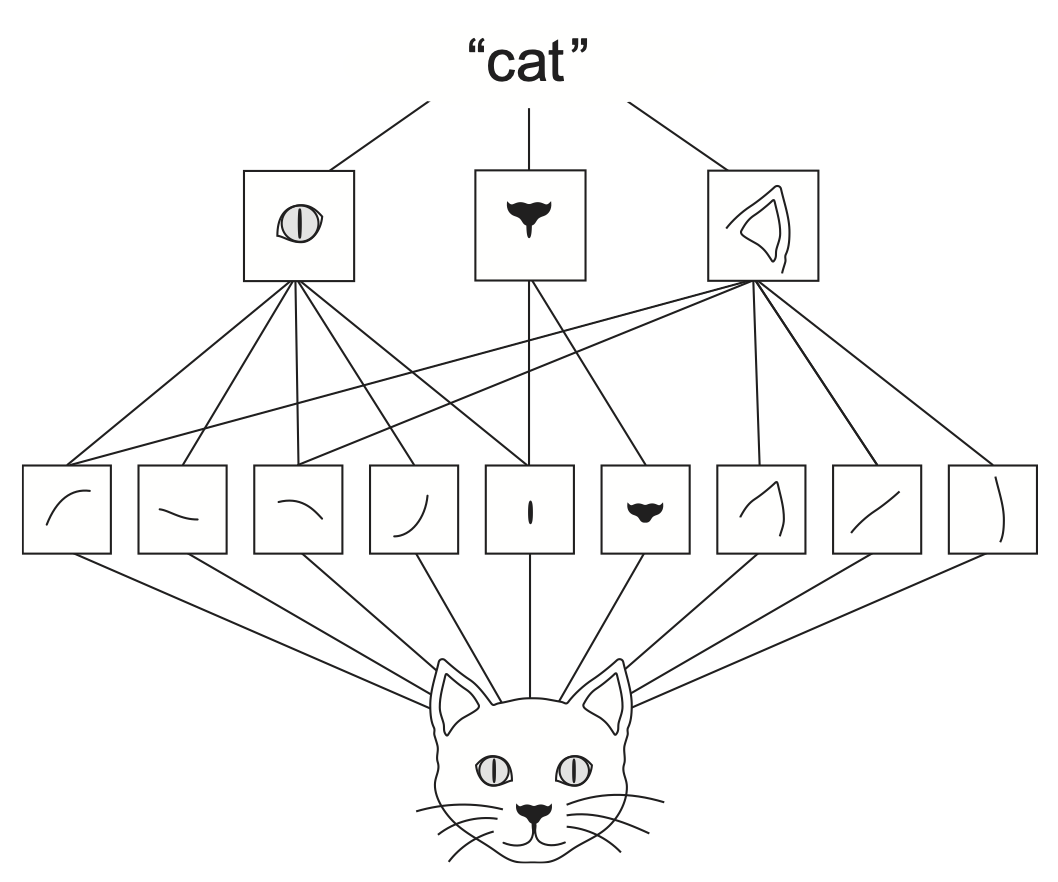
\includegraphics[width=0.7\textwidth]{fig/DLR_Fig_5_2_cat.png}
\caption{The representations of a cat (Chollet and Allair, 2018, Fig 5.2)}
\end{figure}
\pause
\item CNN uses \uured{Convolutional Layers} to learn \uured{parameter efficient} representations
\end{itemize}

}


\frame{\frametitle{Learning Representations for Images (again)}

\begin{figure}[h]
\centering
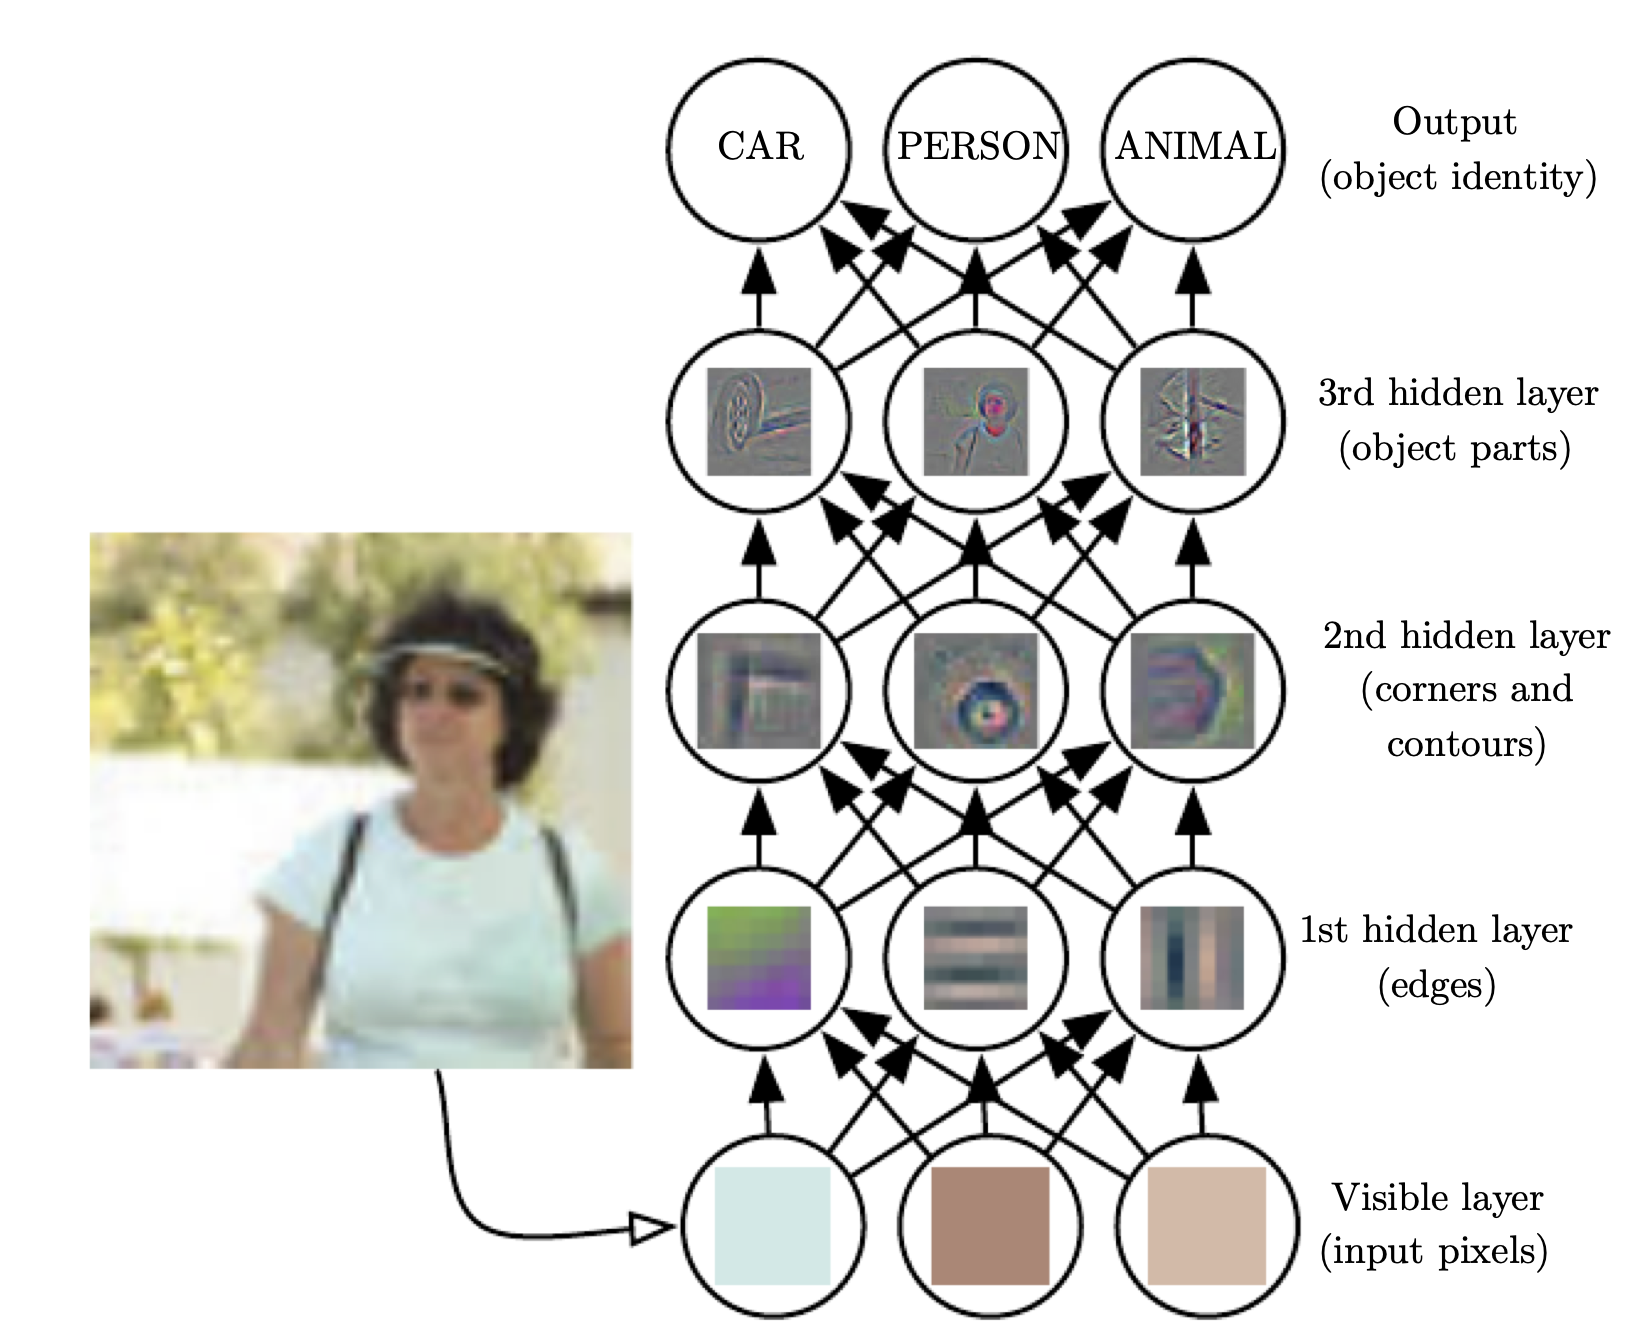
\includegraphics[width=0.8\textwidth]{fig/DL_fig_1_2_representations.png}
\caption{Learning representations for images (Goodfellow et al, 2017, Fig. 1.2)}
\end{figure}

}


\section{Convolution}
\frame{\sectionpage}


\frame{\frametitle{Convolution}

\begin{itemize}
\item Different definitions are common, one example:
\[
y(t) = \int x(\tau) k(t-\tau)d\tau = (x*k)(t)
\]
\item Inutuition: "Weighting together two functions"
\item In a convolutional layer:
\begin{enumerate}
\item $x(t)$: Input
\item $k(t)$: Kernel, filter, "feature"
\item $y(t)$: Output, feature map
\end{enumerate}
\vspace{5mm}
\centering
\href{https://phiresky.github.io/convolution-demo/}{DEMO}

\end{itemize}
}


\frame{\frametitle{Discrete Convolution}

\begin{itemize}
\item If $t$ is discrete (as in a grid):
\[
y(t) = (x*k)(t) = \sum_{\tau=-{\infty}}^{\infty} x(\tau) k(t-\tau)
\]
\pause
\item In the case of images we have 2 discrete dimensions
\[
Y(i,j) = (X * K) \sum_{m} \sum_{n} X(m, n) K(i-m, j-n)
\]
\pause
\item Sometimes the \uured{cross-correlation} is called convolution:
\[
Y(i,j) = (X * K) \sum_{m} \sum_{n} X(m, n) K(i+m, j+n)
\]
\begin{enumerate}
\item $X(i,j)$: Input (2D)
\item $K(i,j)$: Kernel, filter, "feature" (2D)
\item $Y(i,j)$: Output, feature map (2D)
\end{enumerate}
\end{itemize}
}



\frame{\frametitle{Convolution of Images: 2D}
\begin{figure}[h]
\centering
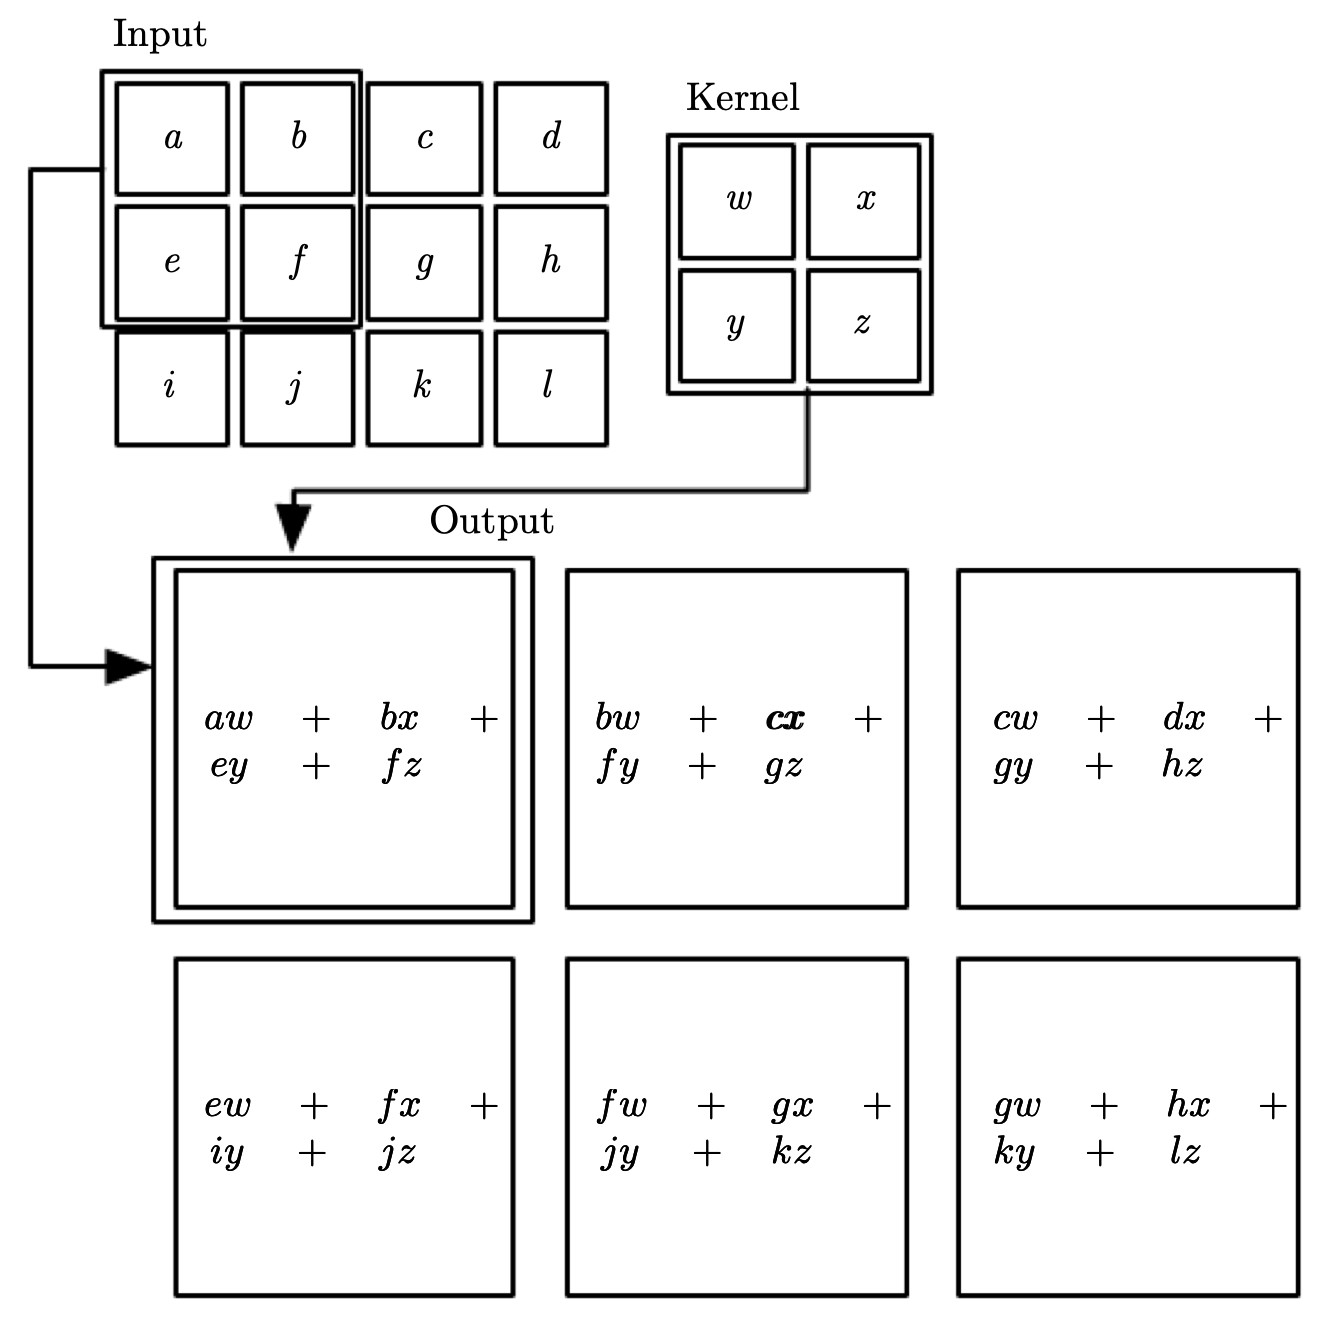
\includegraphics[width=0.8\textwidth]{fig/DL_fig_9_1_conv.png}
\caption{Convolution for an Image (Goodfellow et al, 2017, Fig. 9.1)}
\end{figure}
}

\frame{\frametitle{Convolution of images: Example}
\begin{figure}[h]
\centering
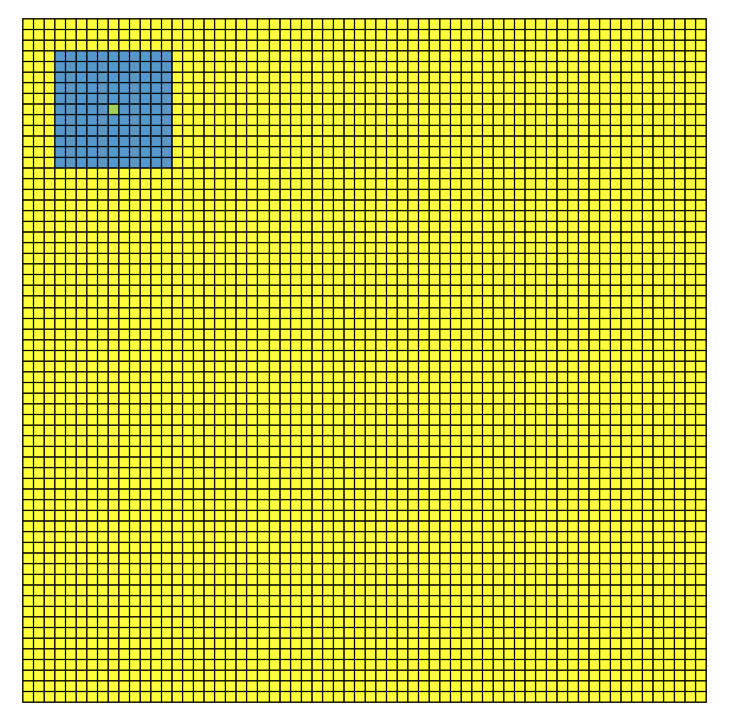
\includegraphics[width=0.8\textwidth]{fig/2d_conv_eklund.png}
\caption{Convolution example.}
\end{figure}
}

\frame{\frametitle{Convolution of images: Examples}
\begin{figure}[h]
\centering
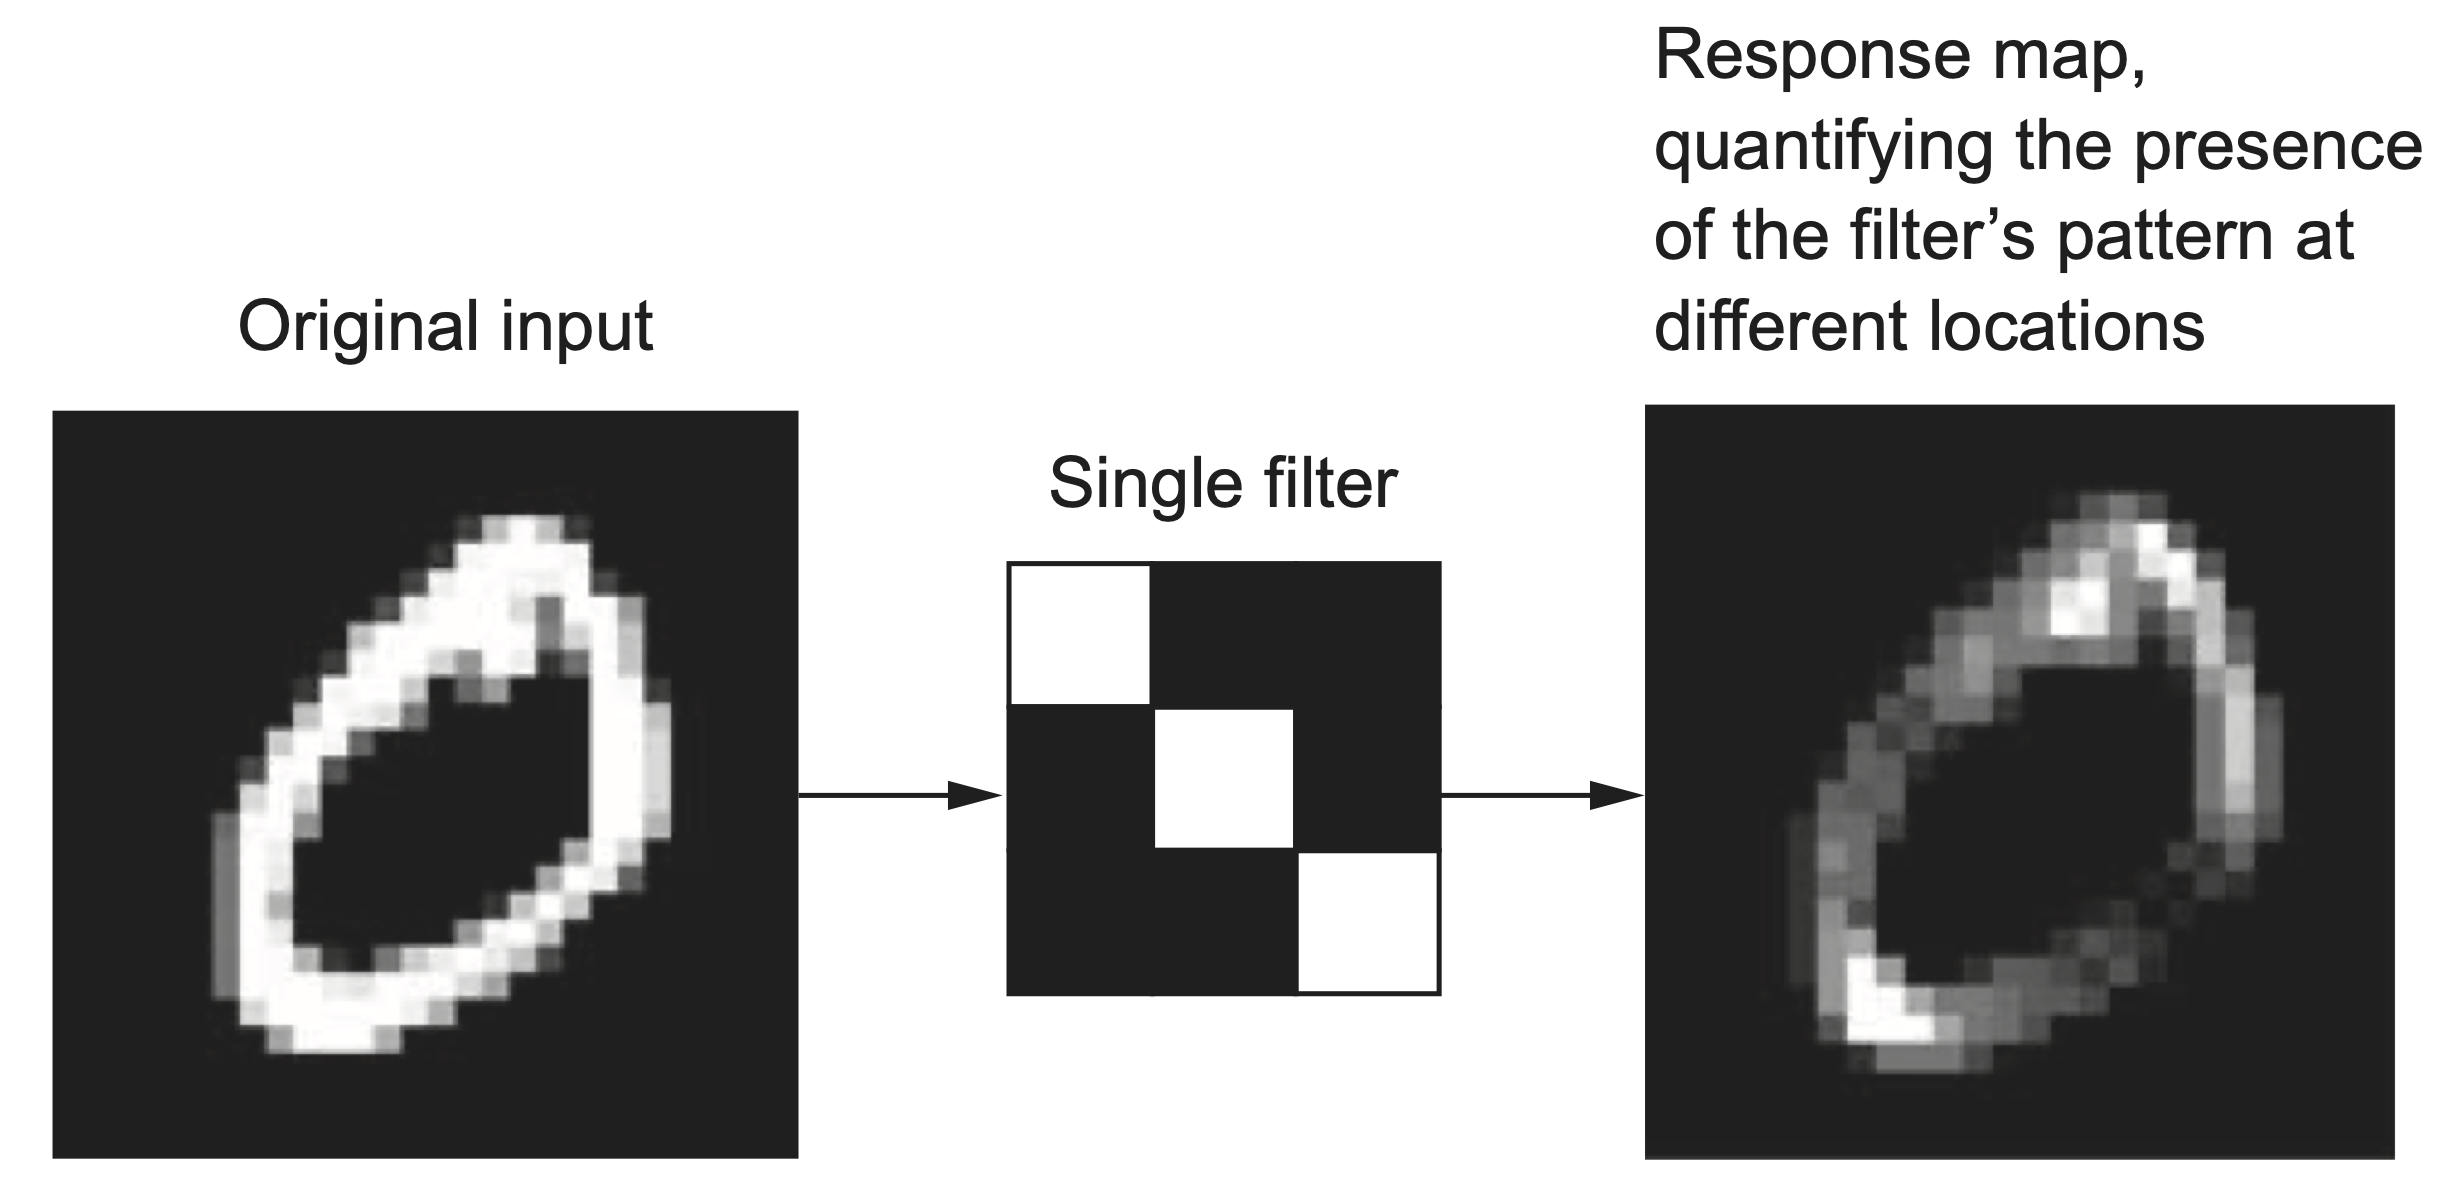
\includegraphics[width=0.8\textwidth]{fig/DLR_fig_5_3_conv_example.png}
\caption{Convolution for an Image (Chollet and Allaire, 2018, Fig. 5.3)}
\end{figure}

}


\frame{\frametitle{Convolution of images: Example}
\[
X=
  \begin{bmatrix}
    0 & 0 & 0 & 1 & 1 \\
    0 & 0 & 0 & 1 & 1 \\
    0 & 0 & 0 & 1 & 1 \\
    0 & 0 & 1 & 1 & 1
  \end{bmatrix}\,,
  K =
  \begin{bmatrix}
    -1 & 1 \\
    -1 & 1
  \end{bmatrix}
\]
\pause
\[
Y=
  \begin{bmatrix}
    0 & 0 & 2 & 0 \\
    0 & 0 & 2 & 0 \\
    0 & 1 & 2 & 0
  \end{bmatrix}\,,
\]
}




\section{Convolutional Neural Networks}
\frame{\sectionpage}

\frame{\frametitle{Convolutional Neural Networks}
\begin{figure}[h]
\centering
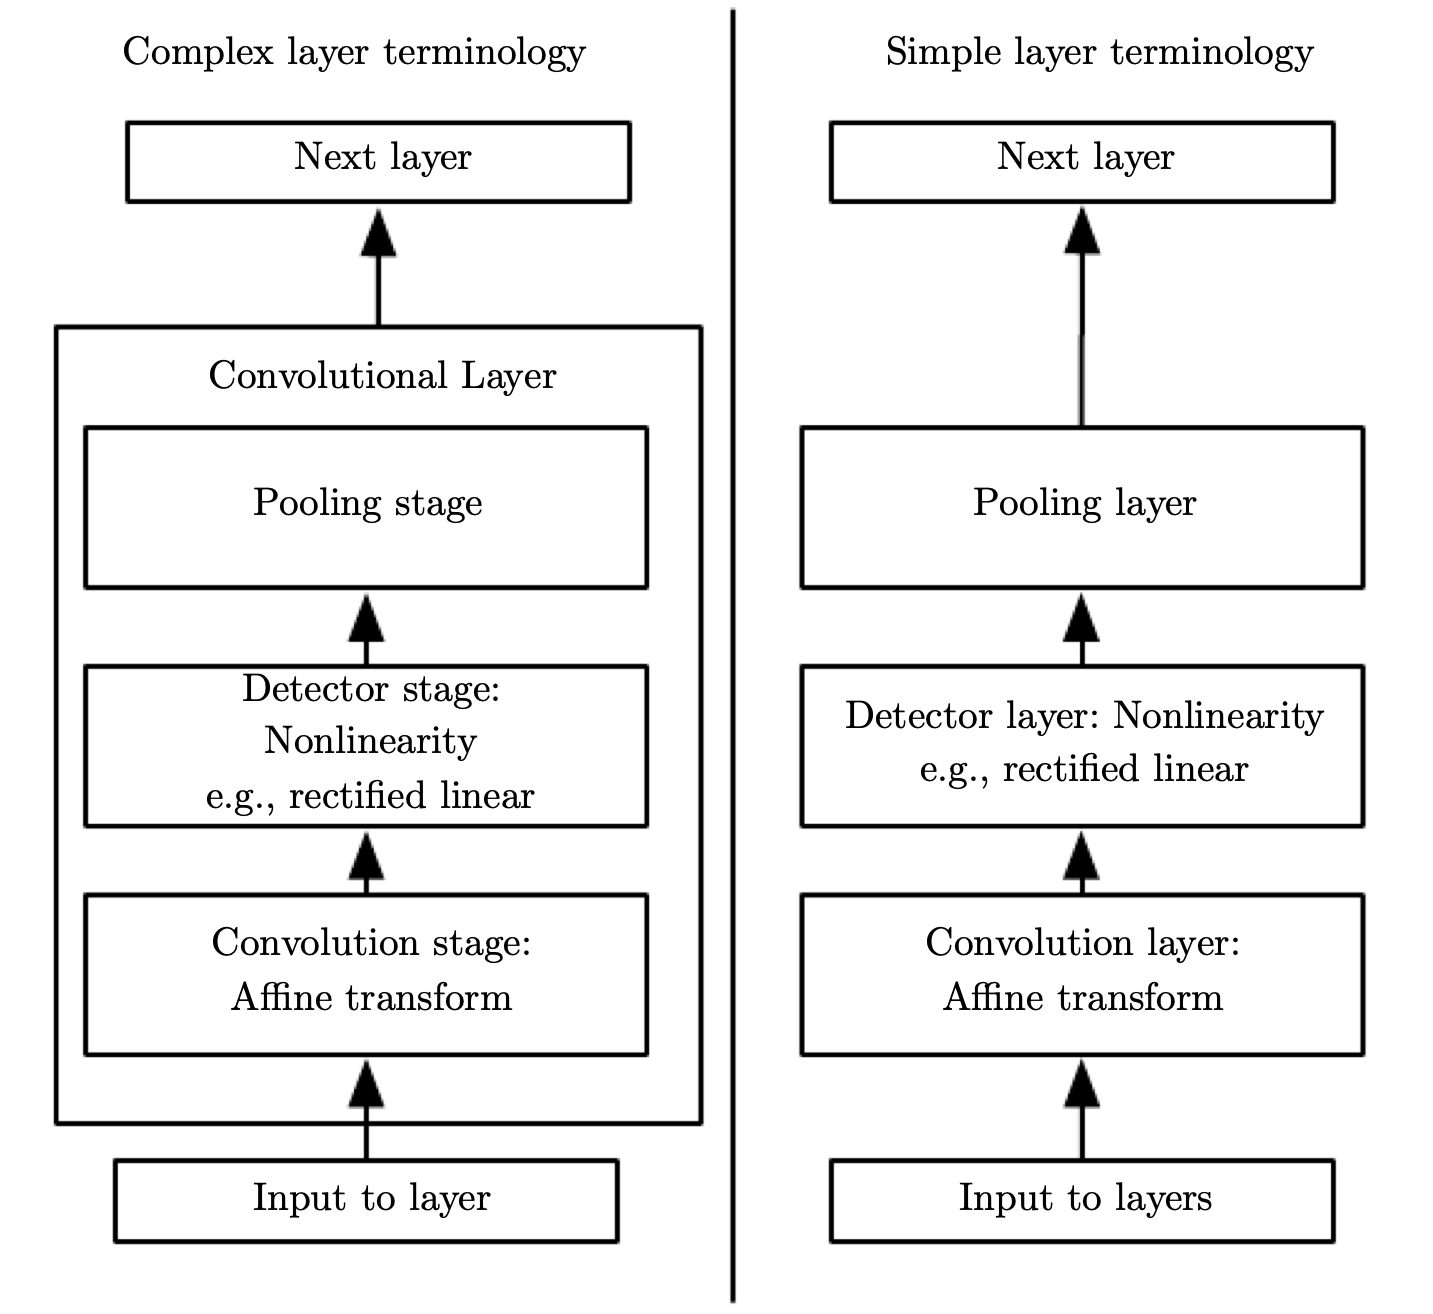
\includegraphics[width=0.8\textwidth]{fig/DL_fig_9_7_conv_layer.png}
\caption{Convolution layer (Goodfellow et al, 2018, Fig. 9.7)}
\end{figure}
}

\frame{\frametitle{Convolutional Neural Networks}

\begin{itemize}
\item Most convolutional neural networks have:
\begin{enumerate}
\item Many convolutional layers
\item More kernels higher up in the network
\item A classification head (usually a feed-forward neural network)
\end{enumerate}
\pause
\item Benefits:
\begin{enumerate}
\item Few(er) parameters (filters)
\item Captures {\color{uured} local structures}
\item Efficient computations\pause
\end{enumerate}
\item How to choose filters?
\begin{enumerate}
\item Before: {\color{uured} manually handcrafted}\pause
\item Now: {\color{uured} learn the filters}
\end{enumerate}

\end{itemize}

}

\subsection{The Convolution Layer}

\frame{\frametitle{Convolution layer}

\begin{itemize}
\item {\color{uured} Input}: Data or Feature Maps
\pause
\item {\color{uured} Parameters}:
\begin{itemize}
\item $N$ filters/kernels of size $m\times m$
\item $N$ bias terms (one per filter)
\end{itemize}
\pause
\item {\color{uured} Activation functions}: Applied element wise on feature maps
\pause
\item {\color{uured} Output}: Feature Maps
\pause
\item In Keras:\\
\texttt{layer\_conv\_2d(filters = 32, kernel\_size = c(3,3), activation = "relu", input\_shape = c(32,32,3))}
\end{itemize}

}

\frame{\frametitle{Padding}

\begin{itemize}
\item Handling {\color{uured} edges}
\item \emph{Padding}: add 0 around the image
\item Nessecary to {\color{uured} keep size} of feature maps
\end{itemize}

}


\frame{\frametitle{Padding}

\begin{figure}[h]
\centering
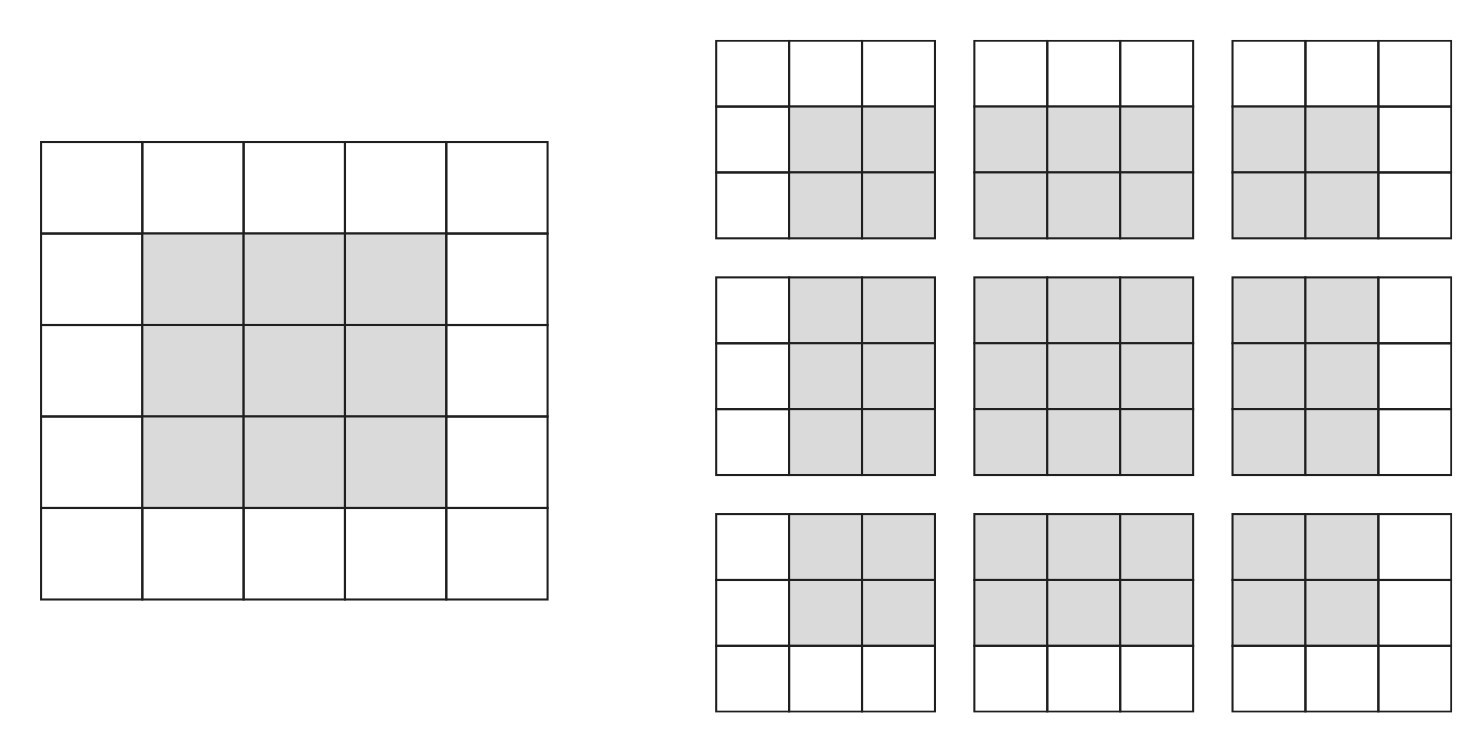
\includegraphics[width=0.8\textwidth]{fig/DLR_fig_5_5_valid.png}
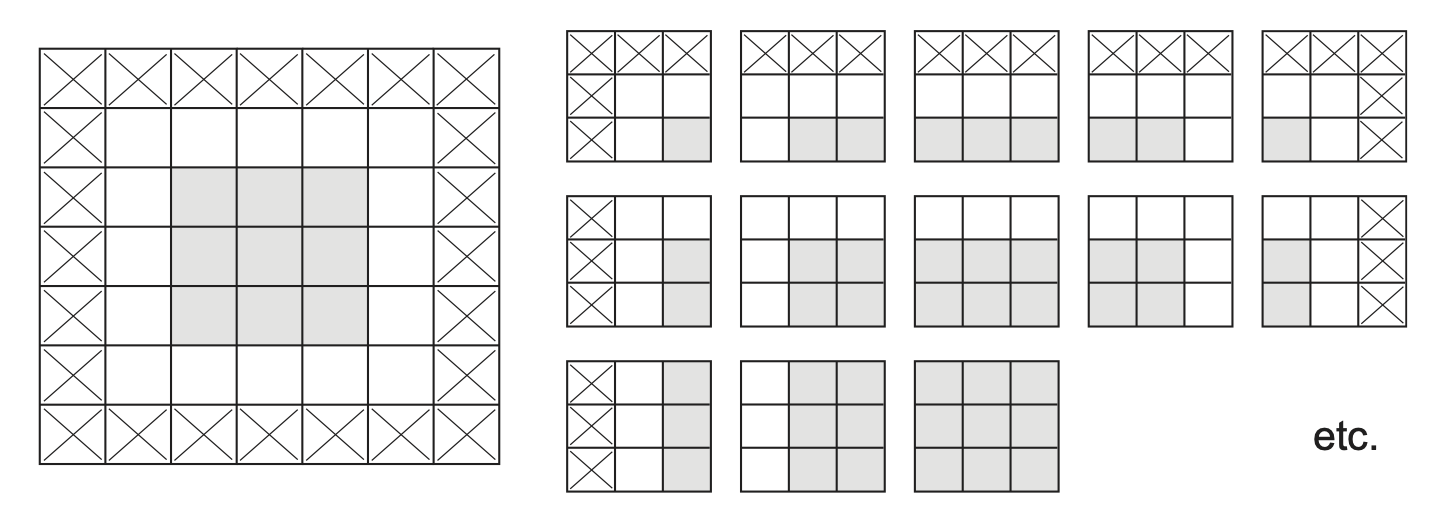
\includegraphics[width=0.8\textwidth]{fig/DLR_fig_5_6_padded.png}
\caption{Padding and valid edge handling (Chollet and Allair (2018), Fig. 5.5, 5.6)}
\end{figure}
}


\frame{\frametitle{Stride}

\begin{itemize}
\item {\color{uured} Skip} every $n$th pixel
\item Reduces the computations
\end{itemize}

\begin{figure}[h]
\centering
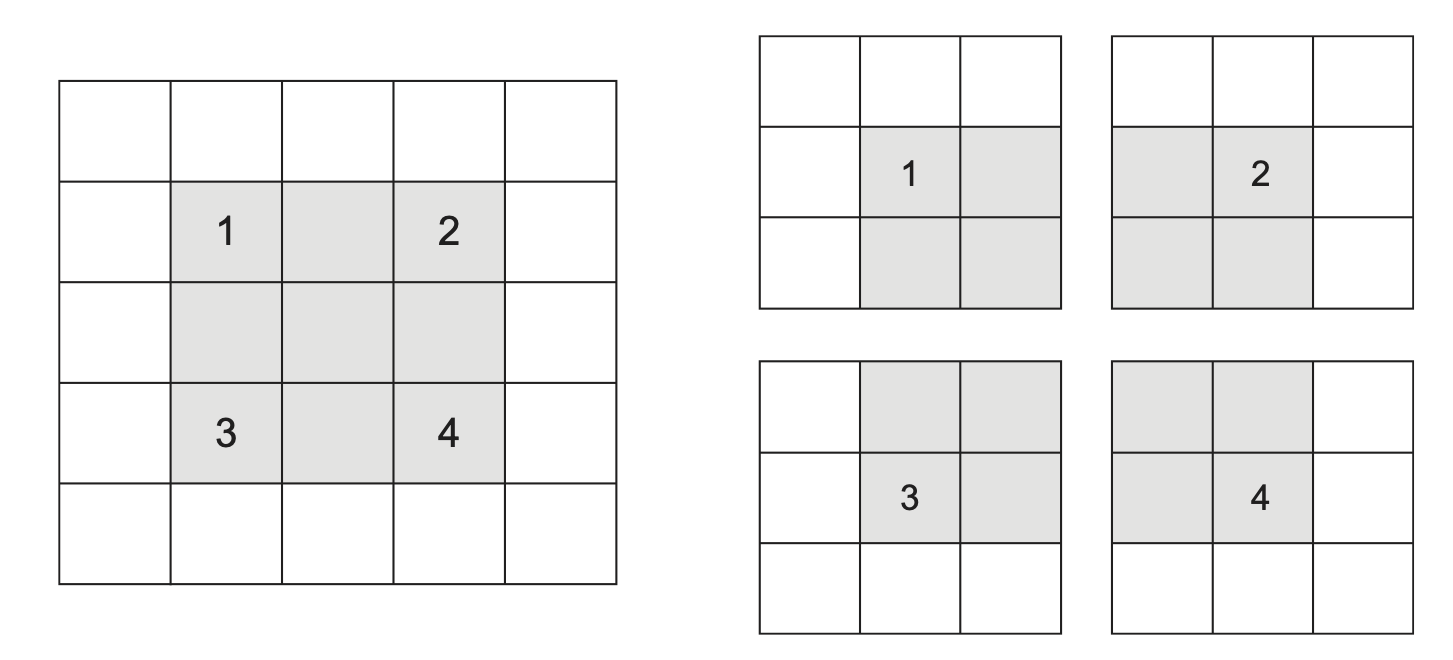
\includegraphics[width=0.8\textwidth]{fig/DLR_fig_5_7_2g2_stride.png}
\caption{Strides (Chollet and Allair (2018), Fig. 5.5, 5.6)}
\end{figure}
}


\frame{\frametitle{Why Convolution Layers?}

\begin{itemize}
\item Captures local spatial structure
\item Reduces the number of parameters (parameter sharing)
\begin{enumerate}
\item The number and size of filters
\item We use the same filters everywhere\pause
\end{enumerate}
\item Example: a 1 megapixel image ($1000 \times 1000$ pixels)
\begin{enumerate}
\item Dense network with 100 nodes: {\color{uured} 100M} parameters
\item CNN network with 100 $3\times 3$ filters: {\color{uured} 1000} parameters \\(900 from filters, 100 bias terms)
\end{enumerate}
\end{itemize}
}

\frame{\frametitle{Convolution Neural Nets}
\begin{figure}[h]
\centering
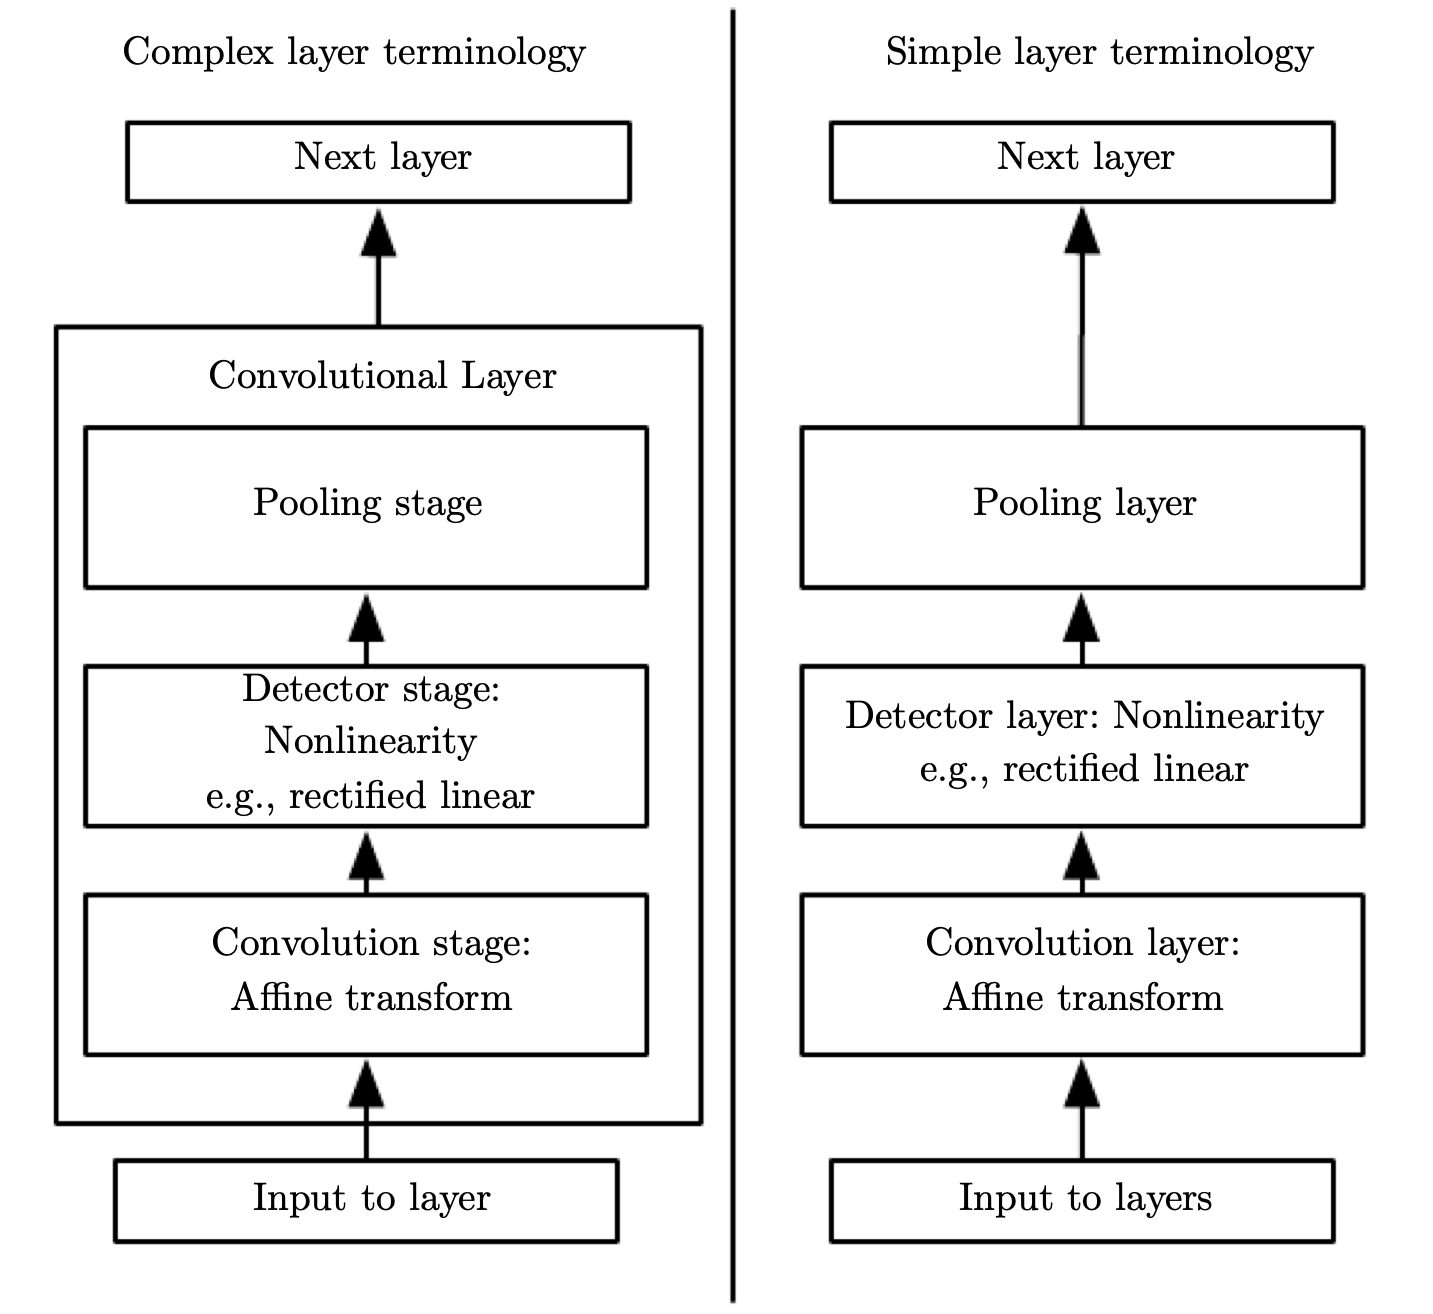
\includegraphics[width=0.8\textwidth]{fig/DL_fig_9_7_conv_layer.png}
\caption{Convolution layer (Goodfellow et al, 2018, Fig. 9.7)}
\end{figure}
}


\frame{\frametitle{Detector stage}

\begin{itemize}
\item Remember, in feed-forward networks: $\mathbf{h} = \sigma(\mathbf{X W}  + b)$
\item In CNN:
\begin{enumerate}
\item $\mathbf{W}$ is the filter\pause
\item $\mathbf{X}$ is the input feature map\pause
\item $\mathbf{X W}$ is the convolutional feature map\pause
\item $b$ is a bias (one per filter) \pause
\item $\sigma$ is the activation function (usually a ReLU)
\end{enumerate}
\end{itemize}

}

\subsection{The Pooling Layer}
\frame{\frametitle{Pooling layer}

\begin{itemize}
\item We take a function $f$ that return one value per pooling kernel\pause
\item Most commonly $f=\max$
\item Commonly a $2\times 2$ pooling kernel with stride 2
\item {\color{uured} Why?} Reduce the size of feature map, but keep the activation\pause
\item In Keras:\\
\texttt{layer\_max\_pooling\_2d(pool\_size = c(2, 2))}(
\end{itemize}

}

\frame{\frametitle{Max Pooling}

\begin{figure}[h]
\centering
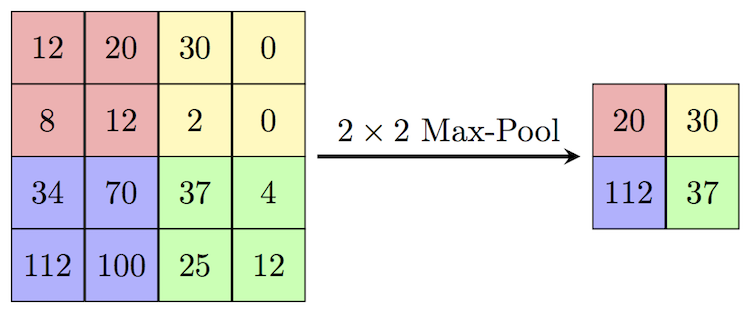
\includegraphics[width=0.8\textwidth]{fig/MaxpoolSample2.png}
\caption{Strides (Computer Science Wikipedia)}
\end{figure}
}

\frame{\frametitle{Using pooling to learn invariances}

\begin{itemize}
\item pooling over spatial positions: invariant to translation
\item pooling over different filters: invariant to transformations
\end{itemize}

\begin{figure}[h]
\centering
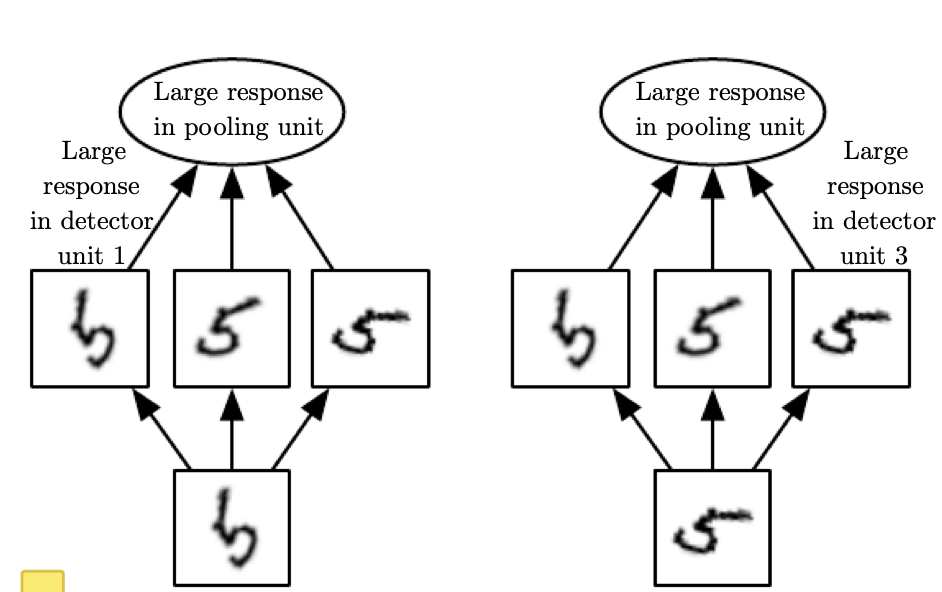
\includegraphics[width=0.7\textwidth]{fig/invariances.png}
\caption{Learning invariances (Goodfellow et al., 2017, Fig. 9.9)}
\end{figure}
}

\subsection{Regularization}

\frame{\frametitle{Data Augmentation}
\begin{figure}[h]
\centering
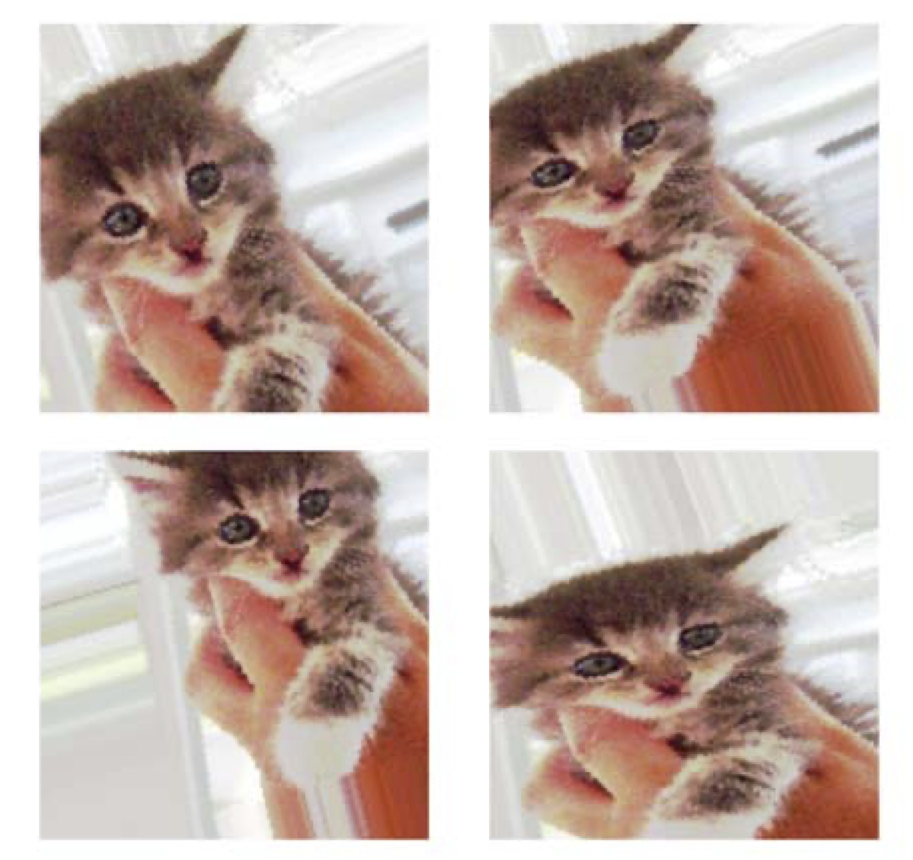
\includegraphics[width=0.6\textwidth]{fig/DLR_fig_5_10_data_augmentation.png}
\caption{Data Augmentation (Chollet and Allair, 2018, Fig 5.10)}
\end{figure}
\pause
\begin{itemize}
\item Can be done directly in Keras (data generator)
\end{itemize}
}


\subsection{Examples}

\frame{\frametitle{Popular CNN architectures}

\begin{itemize}
\item AlexNet (2012), 5 convolutional layers
\item VGG16 (2014), 16 convolutional layers
\item ResNet (2015), 152 convolutional layers
\end{itemize}
}

\frame{\frametitle{VGG16}

\begin{figure}[h]
\centering
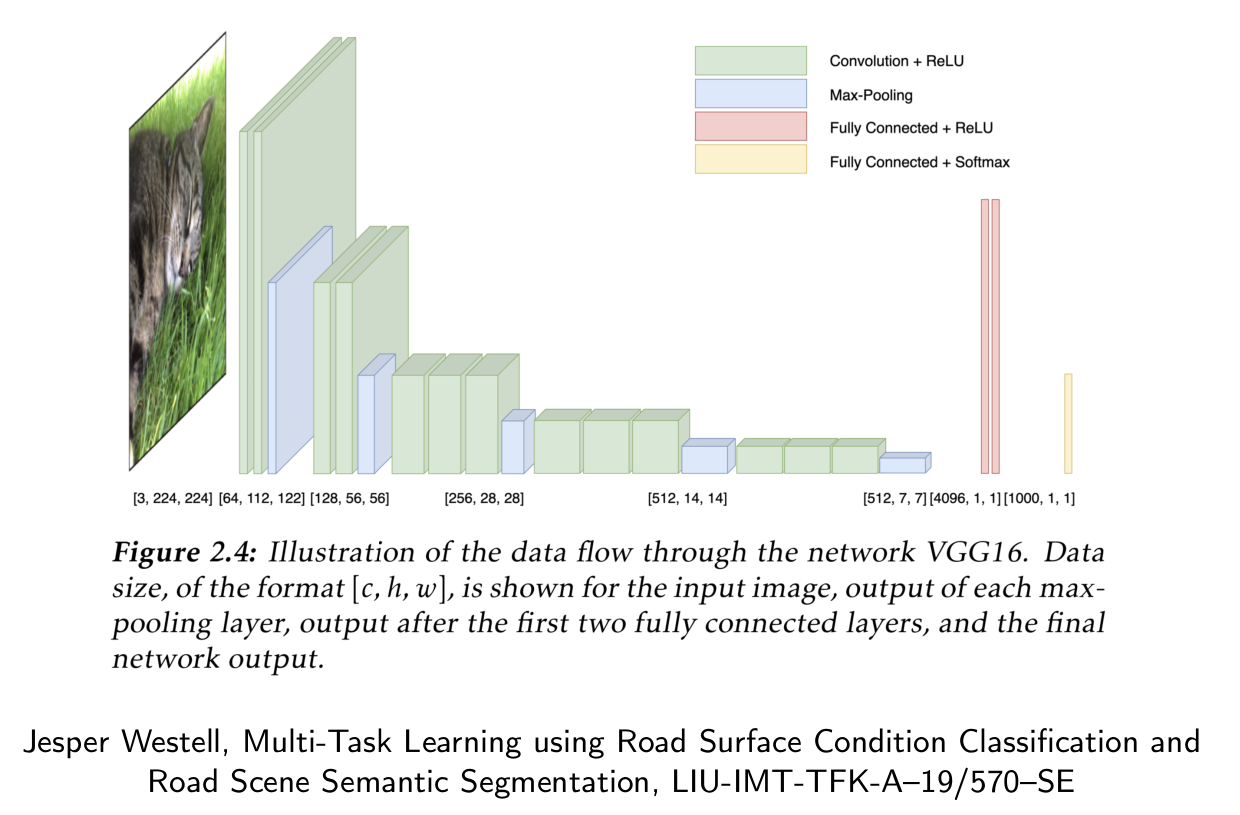
\includegraphics[width=0.9\textwidth]{fig/CNNVGG.png}
%\caption{Strides (Computer Science Wiki: "Max-pooling / Pooling")}
\end{figure}

}

\section{Transfer learning}
\frame{\sectionpage}

\frame{\frametitle{Transfer learning}

\begin{itemize}
\item "{\color{uured} Transfer knowledge} between problems"
\item \uured{Learning representations} in $P_1$ will aid \uured{generalization} in $P_2$\pause
\item A Bayesian perspective: A \uured{strong prior}
\end{itemize}

}



\frame{\frametitle{Learning Representations for Images}

\begin{figure}[h]
\centering
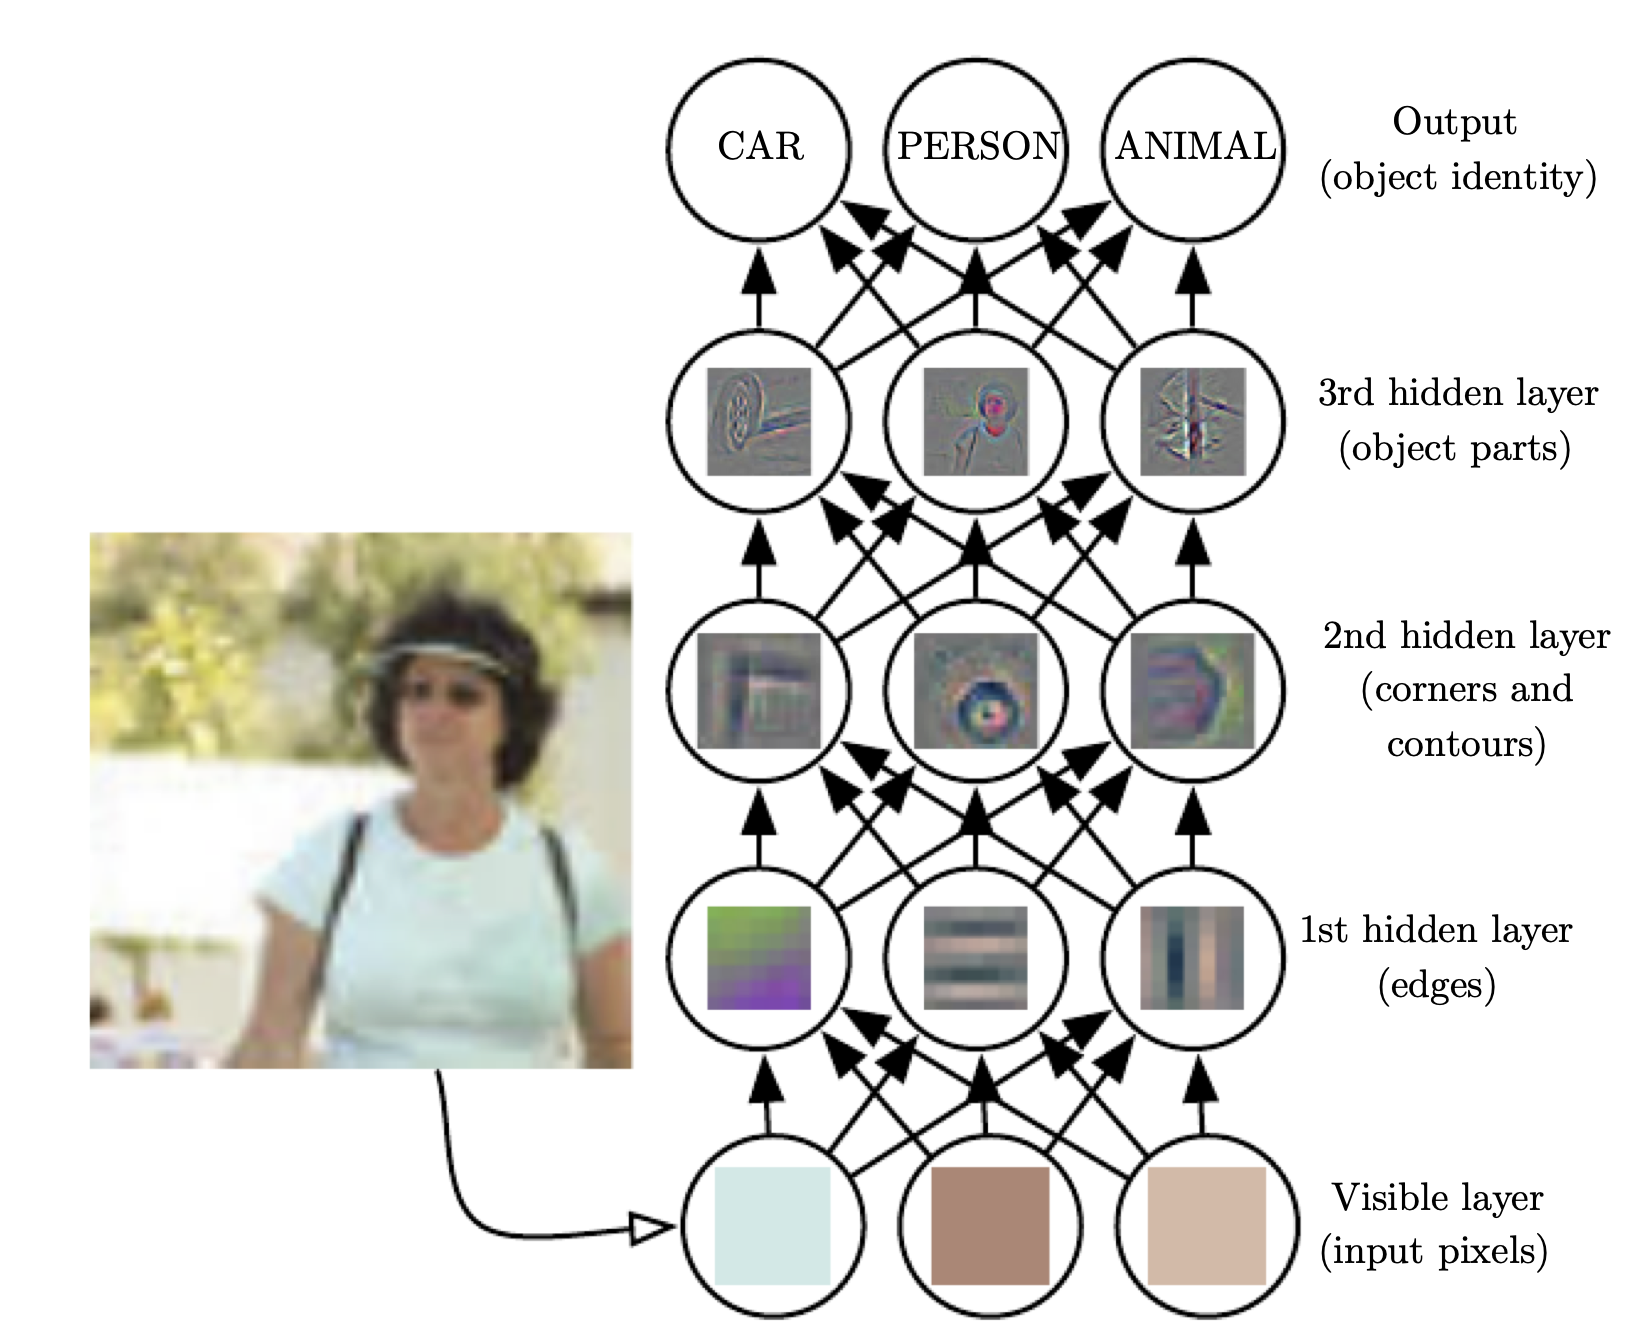
\includegraphics[width=0.8\textwidth]{fig/DL_fig_1_2_representations.png}
\caption{Learning representations can be crucial (Goodfellow et al, 2017, Fig. 1.2)}
\end{figure}

}

\frame{\frametitle{Transfer learning}

\begin{itemize}
\item \uured{In practice}: Transfer/reuse {\color{uured} learned weights} or rather \uured{some weights}\pause
\item Use (large) \uured{pre-trained} models for smaller problems
\item A reason for the success of CNN\pause
\item Two types of transfer learning in Neural Networks:
\begin{itemize}
\item Feature extraction (use pre-trained networks for features)
\item Fine Tuning (adapt pre-trained features)
\end{itemize}
\end{itemize}

}

\frame{\frametitle{Feature Extraction}

\begin{figure}[h]
\centering
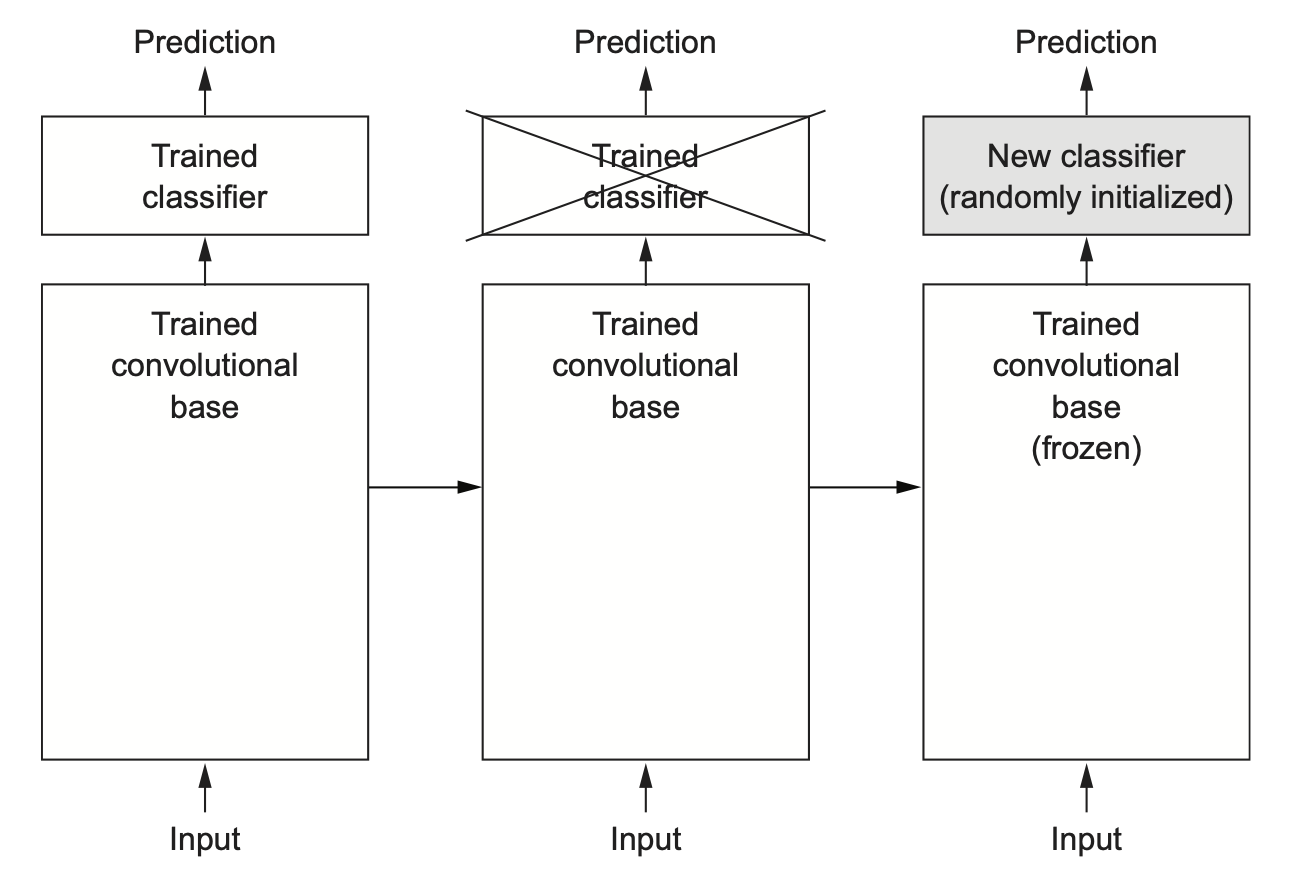
\includegraphics[width=0.8\textwidth]{fig/DLR_fig_5_12_feature_extract.png}
\caption{Using convnets as base for feature extraction (Chollet and Allair, 2018, Fig 5.12)}
\end{figure}

}

\frame{\frametitle{Fine-Tuning}

\begin{figure}[h]
\centering
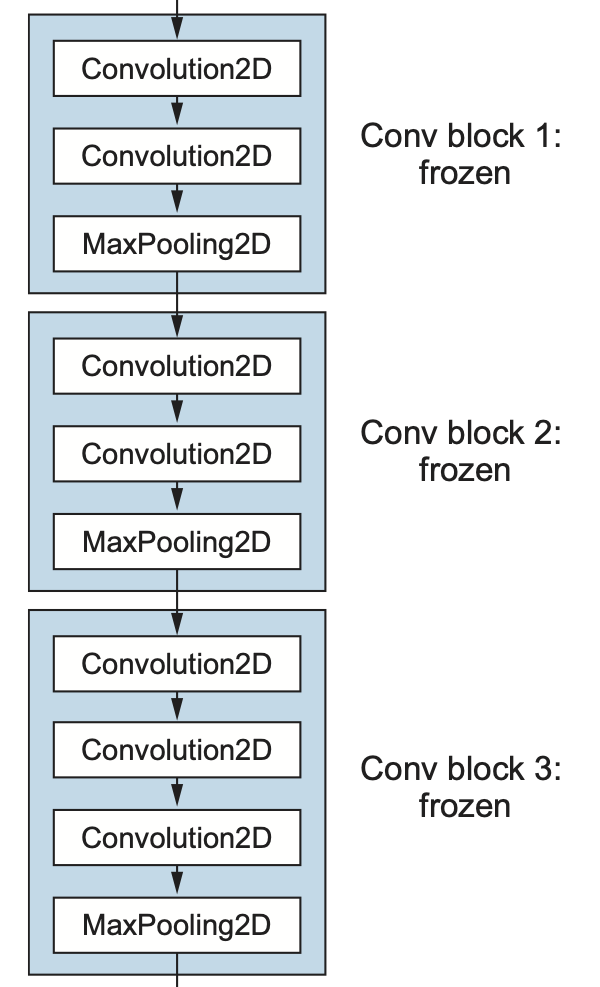
\includegraphics[width=0.45\textwidth]{fig/DLR_fig_5_15_a_fine_tune.png}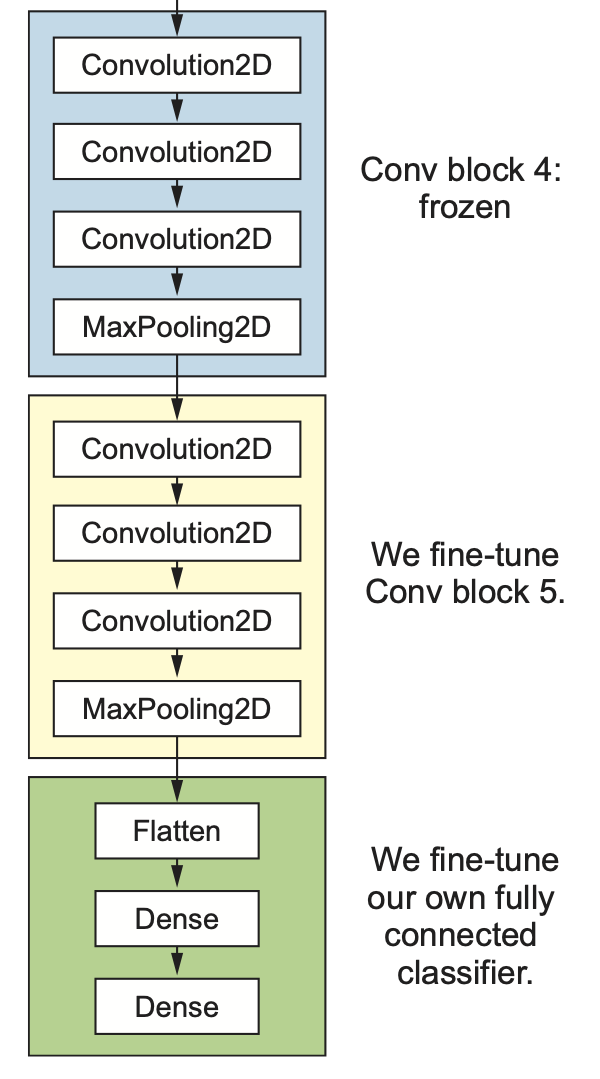
\includegraphics[width=0.45\textwidth]{fig/DLR_fig_5_15_b_fine_tune.png}
\caption{Finetuning a convolutional base (Chollet and Allair, 2018, Fig 5.15)}
\end{figure}

}


\frame{\frametitle{Transfer learning}

\begin{itemize}

\item \uured{Catastophic forgetting} \pause
\item \uured{Domain adaptation}: Same problem but at different input dataset\\ (e.g. language models for legal/medical/political data) \pause
\item \uured{Concept drift}: Similar problem \pause
\item Previously, popular with unsupervised pre-training.
\end{itemize}

}


\section{Practical Methodology}
\frame{\sectionpage}

\frame{\frametitle{Practical Methodology}

\begin{enumerate}
\item Determine your goals\pause
\item Setup your baseline \\(establish a working end-to-end pipeline as soon as possible)\pause
\item Diagnose your networks performance\pause
\item Make incremental improvements
\end{enumerate}

\begin{itemize}
\item \uured{General idea}: Increase data and model capacity until goal is reached\pause
\item \uured{End goal}: Good enough performance on test set
\end{itemize}

}


\frame{\frametitle{1. Determine your goals}

\begin{itemize}
\item Why are you building a model?\pause
\item Set up the metric based on the \uured{overall goal} of the system! \\This may need multiple metrics.\pause %
\item What is good enough? Remember the \uured{Bayes error}!\pause
\item What performance can you expect?\pause
\item Some errors are worse than others, e.g. spam filters.\pause
\item Handling of uncertain predictions:
\item \uured{Coverage}: How large proportions can the system predict?\pause
\item Manual curation can be faster and easier.
\end{itemize}
}

\frame{\frametitle{2. Setup your baseline}

\begin{itemize}
\item Start with...
\begin{itemize}
\item the most simple possible model (logistic regression)\pause
\item previous approaches/baselines\pause
\item a simple neural network that is common in the domain/defaults\\(CNN for images, Adam as optimizer)
\end{itemize}
\end{itemize}
}


\begin{frame}{Remember: Statistical Learning Theory}

\begin{figure}[h]
\caption{Test, training, and model complexity (Goodfellow et al, 2017, Figure 5.3)}
\centering
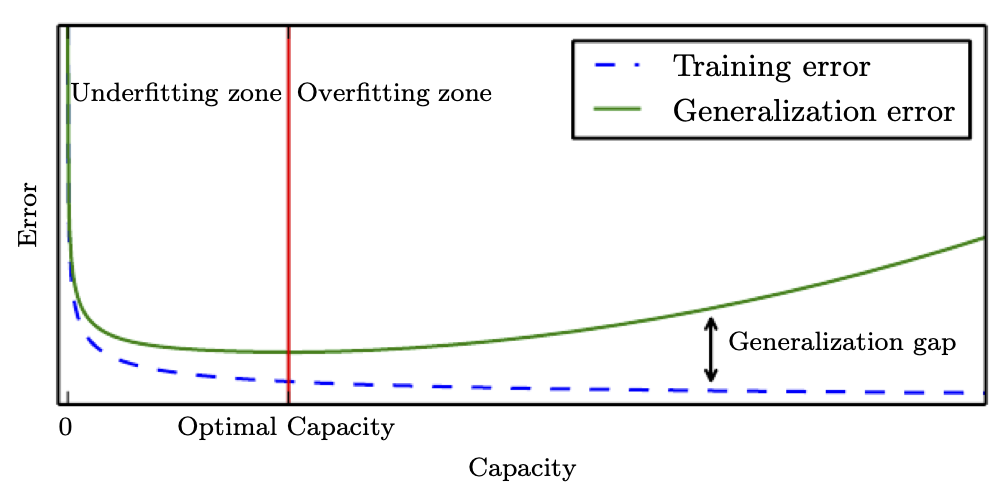
\includegraphics[width=0.8\textwidth]{fig/Dl_5_3.png}
\end{figure}

\end{frame}

\frame{\frametitle{3. Diagnose and improve}

\begin{itemize}
\item High training loss: Training data not fully used\\
Neural network generally performs best when training error is low
\pause
\item High test loss: Low data quality, i.e. large Bayes error?\pause
\item Low training error and high test error: Common situation\pause
\begin{itemize}
\item You can always improve by gather more data, or
\item Regularize to optimal capacity\pause
\end{itemize}
\item \uured{How to know the improvements of additional data?}
\end{itemize}
}

\frame{\frametitle{Learning curve}

\begin{figure}[h]
\centering
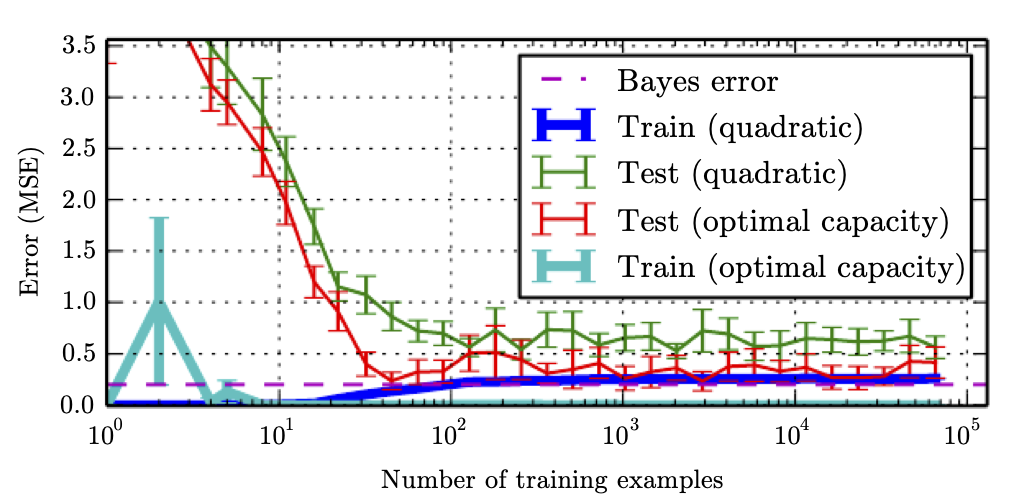
\includegraphics[width=0.8\textwidth]{fig/DL_5_4a.png}
\caption{Learning curve to assess the need for more data (Goodfellow et al., 2017, Fig 5.4)}
\end{figure}

}

\frame{\frametitle{3. Diagnosing and improving your model: Regularization}

\begin{itemize}
\item Best performance: Larger model that is regularized well.
\item Warning: Avoid \uured{the algorithm rabbit hole}\pause
\item Adapt hyperparameters to get \uured{optimal capacity}\pause
\item Hyperparameter Search Goal: \\adjust the model capacity to match the complexity of the task.\pause
\item Marginal hyperparameter has a U-shaped error function (ideally)\pause
\item Neural Networks Steps:
\begin{enumerate}
\item Get good training error. E.g. by tune learning rate and increasing capacity\pause
\item Tune hyperparameters (regularization):\\
Requires monitoring both training and test error
\end{enumerate}
\end{itemize}
}

\frame{\frametitle{Hyper-parameter optimization}

\begin{itemize}
\item Neural networks has many hyperparameters
\item \uured{What is a hyperparameter in a neural network?}\pause
\item Grid search:
\begin{itemize}
\item Setup a grid of potential values
\item For 1-4 hyperparameter: grid search can work well
\item Usually iterative/repeated grid search is best: start with three values, and work iteratively
\item Grows exponentially with the number of parameters
\end{itemize}
\pause
\item Random search
\begin{itemize}
\item Specify a marginal distribution for each hyperparameter (additional work)
\item Common: uniform on log scale
\item Can also be done iteratively
\item Can be exponentially more efficient
\item Generally reduce the error faster in setting with many hyper parameters
\end{itemize}
\end{itemize}
}

\frame{\frametitle{Diagnosis and Debugging}

\begin{itemize}
\item Visualize the model predictions\pause
\item Analyze the worst errors: \uured{why?}\pause
\item Use train and test error as a diagnostic: \uured{Can you overfit the data?}\pause
\item Use test suites: Can you get known results on a toy data. Both training error and derivatives\pause
\item Monitor the gradients\pause
\item Monitor activation function statistics. Are some never activated?
\end{itemize}
}

\end{document}
